\section{Advent Nopele Olansi Damiahan Sihite (1174089)}
\subsection{Buku}
Rp.0 (Belum Lunas)
\subsection{Sejarah}
\begin{itemize}

	\item35000 tahun yang lalu, di dinding gua Lascaux, Perancis, para pemburu Cro-Magnon menggambar hewan mangsa mereka, juga garis yang dipercaya sebagai rute migrasi hewan-hewan.
	\item	Pada tahun 1700-an teknik survey modern untuk pemetaan topografis diterapkan, termasuk juga versi awal pemetaan tematis, misalnya untuk keilmuan atau data sensus.
	\item	Awal abad ke-20 memperlihatkan pengembangan “litografi foto” dimana peta dipisahkan menjadi beberapa lapisan (layer). Perkembangan perangkat keras komputer yang dipacu oleh penelitian senjata nuklir membawa aplikasi pemetaan menjadi multifungsi pada awal tahun 1960-an.
	\item	Tahun 1967 merupakan awal pengembangan SIG yang bisa diterapkan di Ottawa, Ontario oleh Departemen Energi, Pertambangan dan Sumber Daya, Digunakan untuk menyimpan, menganalisis dan mengolah data.
	\item	GIS dengan gvSIG.CGIS merupakan sistem pertama di dunia dan hasil dari perbaikan aplikasi pemetaan yang memiliki kemampuan timpang susun (overlay), penghitungan, pendijitalan/pemindaian (digitizing/scanning), mendukung sistem koordinat national yang membentang di atas benua Amerika.
	\item	CGIS bertahan sampai tahun 1970-an dan memakan waktu lama untuk penyempurnaan setelah pengembangan awal, dan tidak bisa bersaing denga aplikasi pemetaan komersil yang dikeluarkan beberapa vendor seperti Intergraph.


\end{itemize}
\subsection{Link}
http://tiny.cc/rodhez
\subsection{Plagiarism}'\begin{figure}[H]
	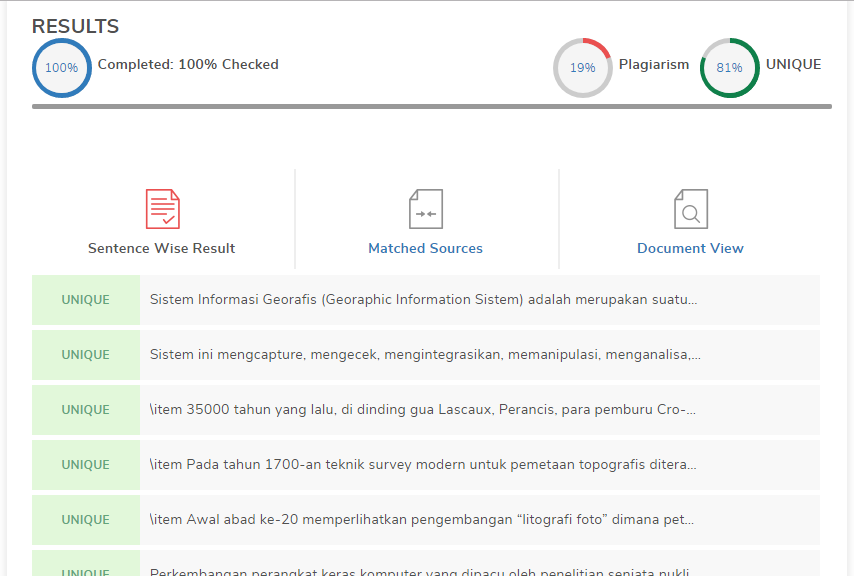
\includegraphics[width=8cm]{figures/Tugas1/1174089/plagiarisme.png}
	\centering
	\caption{Plagiarisme.}
\end{figure}	

\subsection{Cara Penggunaan}
\subsubsection{Gambar}

\hfill\break


Contoh Gambar
\begin{figure}[H]
	
\includegraphics[width=4cm]{figures/himatif.png}
	\centering
	\caption{Contoh gambar.}
\end{figure}

\subsubsection{List}
\begin{enumerate}
	\item Satu
	\item Dua
\end{enumerate}

\begin{itemize}
	\item Satu
	\item Dua
\end{itemize}

